\chapter{Autograding}\label{ch:assignments}

Much of this chapter will be assuming that you are using the Anubis Management IDE. These are special
Anubis Cloud IDEs \ref{ch:cloud_ides} that have the CLI and docker packaged into them. These
IDEs are only available to course admins.

\section{Assignment Structure}\label{sec:assignment-structure}

Under Anubis each student gets their own github repository for each assignment.
When they push to their repo, Anubis sees the push event and runs tests on their code.
The results are then available to students on the Anubis website in real time.
Under this model students can push as many times as they would like before the assignment deadline.

Assignment repositories are created from template repositories.
TAs or professors can set up a repo with the necessary files or starter code for students to work on.
Template repositories can be set up in such a way that constrains student code.
With C or C++ assignments, adding some starter files with a Makefile constrains students
to all start from the same point.
Instead of getting \textit{N} submissions all with different file names and run options,
everyone's code will compile and run with the same commands.
This structure makes automating tests trivial and effective.

\section{Creating Autograde Tests}\label{sec:creating-autograde-tests}

Using the anubis cli, you can initialize a new assignment using
\mint{shell}|anubis assignment init <name of assignment>|

The first file you will want to edit is the \textit{meta.yml} that gets created.
This is where things like the assignment name, and due dates should be defined.
There is also a generated unique code that anubis uses to identify this assignment.
Hold on to this, as we will use it in the next step.

\begin{minted}{yaml}
assignment:
  name: "OS Final Exam"
  class: "CS-UY 3224"
  hidden: false

  # Optionally specify the github classroom link
  # for students to get their repo.
  #
  #  !! Remember to set the Custom repository
  #  !! prefix to {name}-{unique_code}
  #  !! when creating the assignment on
  #  !! Github Classroom
  github_classroom_url: "...."

  # Don't change these!
  unique_code: "839f70b2"
  pipeline_image: "registry.digitalocean.com/anubis/assignment/{unique_code}"

  # Specify the important dates here
  # * Remember! These are interpreted as America/New_York *
  date:
    release: "2021-05-17 06:00:00"
    due: "2021-05-19 06:00:00"
    grace: "2021-05-19 06:30:00"

  # This description will be shown to the user on the Anubis website.
  description: |
    Good luck.
\end{minted}

Here is an example generated meta.yml from the OS final exam this semester.
The only fields that you will need to fill in are the github classroom url.
This is the URL that is given to you when you create a github classroom assignment.
That link will then be provided as a button for students to click on the Anubis website.


\section{Writing Autograde Tests}\label{sec:writing-autograde-tests}

All the files to build and run a complete anubis pipeline image will be dropped into the new directory.

\begin{minted}{text}
new-assignment
|- assignment.py
|- Dockerfile
|- meta.yml
|- pipeline.py
|- test.sh
`- utils.py
\end{minted}

The only thing you will ever need to edit is assignment.py.
This is where you define your build and test code.
Just like all the other cool libraries out there, the anubis pipeline works
through hooking functions.
Here is a minimal example of an assignment.py that will build and run a single simple test.

\begin{minted}{python}
from utils import register_test, register_build, exec_as_student
from utils import (
    TestResult, BuildResult, Panic, DEBUG,
    xv6_run, did_xv6_crash,
    verify_expected, search_lines, test_lines
)

@register_build
def build(build_result: BuildResult):
    stdout, retcode = exec_as_student('make xv6.img fs.img')

    build_result.stdout = stdout.decode()
    build_result.passed = retcode == 0


@register_test('test echo')
def test_1(test_result: TestResult):
    test_result.stdout = "Testing echo 123\n"

    # Start xv6 and run command
    stdout_lines = xv6_run("echo 123", test_result)

    # Run echo 123 as student user and capture output lines
    expected_raw, _ = exec_as_student('echo 123')
    expected = expected_raw.decode().strip().split('\n')

    # Attempt to detect crash
    if did_xv6_crash(stdout_lines, test_result):
        return

    # Test to see if the expected result was found
    verify_expected(stdout_lines, expected, test_result)
\end{minted}

There are a couple functions to point out here.
The \textit{register\_build} and \textit{register\_test} decorators are how
you tell anubis about your build and test.
The \textit{exec\_as\_student} function is how you should call any and all student code.
It lowers the privileges way down so that even if the student pushes something
malicious, they are still low privileged enough where they cannot do much.
It also adds timeouts to their commands.
Boxing student code in like this is absolutely essential.
Do not underestimate the creative and surprising ways students will find to break things.

Each test is passed a \textit{test\_result} object.
This object has 3 fields.
All you need to do is set the fields on the \textit{test\_result} object.
The results will then be reported to the anubis api, and then to the student.

\begin{minted}{python}
class TestResult(object):
    def __init__(self):
        # The standard out for the students tests. You can
        # add extra text in this field as needed.
        self.stdout: str = None

        # The message is an optional parameter that will
        # insert a short message in bold above the standard
        # out on the website frontend.
        self.message: str = None

        # Passed should be a boolean value. True if the test
        # passed, and False if it did not.
        self.passed: bool = None
\end{minted}

The functions \textit{run\_xv6} and \textit{did\_xv6\_crash} are very specific to the Intro to OS needs.
There are also some general functions that are just as helpful.

\begin{minted}{python}
def exec_as_student(cmd, timeout=60) -> typing.Tuple[bytes, int]:
    """
    Run a command as the student. Any and all times that student
    code is run, it should be done through this function. Any other
    way would be incredibly insecure.

    :param cmd: Command to run
    :param timeout: Timeout for command
    :return: bytes output, int return code
    """


def verify_expected(
    stdout_lines: typing.List[str],
    expected_lines: typing.List[str],
    test_result: TestResult,
    case_sensitive: bool = True,
    search: bool = False
):
    """
    Check to lists of strings for quality. Will strip off whitespace from each line
    before checking for equality. The stdout_lines should be from the student code.
    The expected_lines should then be whichever lines are expected for this test.

    * The fields on the test_result object will be set automatically based on if the
    expected output was found. *

    :param stdout_lines: students lines as a list of strings
    :param expected_lines: expected lines as a list of strings
    :param test_result: TestResult object for this test
    :param case_sensitive: boolean to indicate if the comparison should be case sensitive
    :param search: boolean to indicate if the stdout should be searched instead of
                   directly compared for equality
    :return:
    """


def test_lines(
        stdout_lines: typing.List[str],
        expected_lines: typing.List[str],
        case_sensitive: bool = True
) -> bool:
    """
    Test lines for exact equality. Whitespace will be stripped off each line automatically.

    * Optionally specify if the equality comparison should be case sensitive *

    >>> test_lines(['a', 'b', 'c'], ['a', 'b', 'c']) -> True
    >>> test_lines(['a', 'debugging', 'b', 'c'], ['a', 'b', 'c']) -> False
    >>> test_lines(['a', 'b'],      ['a', 'b', 'c']) -> False

    :param stdout_lines: students standard out lines as a list of strings
    :param expected_lines: expected lines as a list of strings
    :param case_sensitive: optional boolean to indicate if comparison should be case sensitive
    :return: True if exact match was found, False otherwise
    """


def search_lines(
        stdout_lines: typing.List[str],
        expected_lines: typing.List[str],
        case_sensitive: bool = True
) -> bool:
    """
    Search lines for expected lines. This will return true if all expected lines are in the
    student standard out lines in order. There can be interruptions in the student standard out.
    This function has the advantage of allowing students to still print out debugging lines
    while their output is still accurately checked for  the expected result.

    >>> search_lines(['a', 'b', 'c'], ['a', 'b', 'c']) -> True
    >>> search_lines(['a', 'debugging', 'b', 'c'], ['a', 'b', 'c']) -> True
    >>> search_lines(['a', 'b'],      ['a', 'b', 'c']) -> False

    * Optionally specify if the equality comparison should be case sensitive *

    :param stdout_lines:
    :param expected_lines:
    :param case_sensitive:
    :return:
    """
\end{minted}


\section{Deploying Autograde Tests}\label{sec:deploying-autograde-tests}


Once you have tests written, then it is time to push them to Anubis.
The next thing that needs to be done is push the image to the docker registry and
upload the assignment data to anubis.
This is as simple as running two commands:

\begin{minted}{shell}
# sends assignment metadata to anubis api
anubis assignment sync

# builds then pushes the assignment
# pipeline image to the registry
anubis assignment build --push
\end{minted}


\section{Submission Pipelines}\label{sec:submission-pipelines}

\begin{figure}[ht]
    \centering
    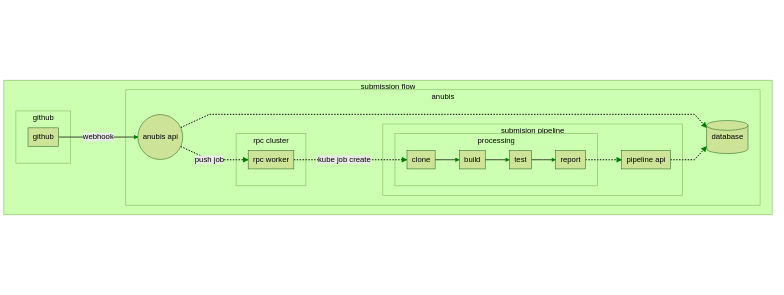
\includegraphics[width=1\textwidth]{figures/submission-flow.mmd.png}
    \caption{Submission Pipelines are a complex multi service data flow. \label{fig:submission-flow} }
\end{figure}

Submissions Pipelines~\fref{fig:submission-flow} are where the autographing is really happening.
When students push code to their github repositories, Anubis sees the new
commits and creates a pipeline job.
Each commit to student github repository gets a new Submission Pipeline.

\subsection{Kubernetes Job}\label{subsec:kubernetes-job}

Each Submission Pipeline is a \href{https://kubernetes.io/docs/concepts/workloads/controllers/job/}{Kubernetes Job}.
There are certain assurances that can be made when using Kubernetes Jobs.
If there is an issue on one node on the cluster that prevents a submission job from finishing,
Kubernetes will reschedule and retry the Submission Pipeline elsewhere.

\subsection{Pipeline State Reporting}\label{subsec:pipeline-state-reporting}

Some assignment tests will also take a long time to process each submission.
Due to this reality, live state updating was added to the Submission Pipelines.

There is an internal REST api that is only for submission pipelines to report state to.
This pipeline is called the \textit{pipeline-api}.
The \textit{pipeline-api} is specifically a subset of the main api.
It has different view functions defined for it.
The purpose of these special api servers is to take state updates from submission
pipelines and update the database.

If a submission is processing the website will poll for updates.
This complex multi service state reporting model is how results from isolated
submission pipelines appear on the website for students as they happen.

\subsection{Pipeline Stages}\label{subsec:pipeline-stages}

It is important to note that at each stage of the submission pipeline,
we will be moving execution back and forth between two unix users.
There will be the entrypoint program managing the container as user \textit{anubis}.
The \textit{anubis} user will have much higher privileges than the \textit{student} user.
The \textit{student} user will be used whenever executing student code.
It will not have any level of access to anything from the \textit{anubis} user.

\subsubsection{Clone}

In this initial stage, we will pull the current repo down from github.
After checking out the commit for the current submission, we will also delete
the \textit{.git} directory as it is not needed.
Lastly we will chown the entire repo as \textit{student:student}.
This will then be the only place in the container that the student user
can read or write to (other than /tmp of course).

\subsubsection{Build}

At this stage we hand execution off to student code for the first time.
Code must be built as the student user.
The function that was marked with the \textit{register\_build} decorator handles this phase.
The stdout and return code of the build will be captured by the \textit{anubis} user.
For most assignments, the success of the build is determined by the return code.
No extra parsing of the stdout should be necessary.

\subsubsection{Test}

Tests are defined on a per-assignment basis.
Again, student code will be executed for this step.
That code must be executed as the \textit{student} user.

Each test is defined as a python function that was decorated with the
\textit{register\_test} decorator.
The function should run the student code for whatever they are testing, then
confirm that the standard out matches whatever was expected.

The state updating at this step is automatic.
After each test hook is called, the results will automatically be sent off to the
\textit{pipeline-api}.

After the last test is called, the pipeline sends a special state update stating that
the submission tests have completed.
It is important that this step happens as it is where the submission is marked as
processed.

\subsection{A Word on Isolation}\label{subsec:a-word-on-isolation}


We are executing student code in the submission pipeline containers.
Due to this reality, the pipelines are designed from the ground
up to be isolated in whatever way they can be.

There is a special
\href{https://kubernetes.io/docs/concepts/services-networking/network-policies/}{kubernetes network policy}
that is applied to  all the submission pipeline pods.
This policy limits the pod to only being able to connect to the \textit{pipeline-api} service.
Using simple resource requests and limits in kubernetes enables
limits on resources like cpu and memory.

In early versions of Anubis, there were not memory limits on submission
containers. 
Several students would push code that would blow up in memory. 
These students were not acting malicious, they just did not understand
how memory works in C that well.
When this would happen, the node would be quickly drained of available memory,
and the OOM killer would start taking other processes and containers down.
Obviously this lead to sensible resources limits being placed
on student code. In more modern versions of Anubis there is proper isolation and
resource limits that are placed on students.


